\documentclass[11pt]{article}
% \usepackage{amsmath}
\usepackage{mymacros}
\usepackage[utf8]{inputenc}
\usepackage[margin=0.75in]{geometry}

\title{CSC111 Project 2 Report: Tree-Based Equation Solver}
\author{Areez Chishtie}
\date{\today}

\begin{document}
\maketitle

\section*{Problem Description and Research Goal}

There are many tools available online for solving various classes of equations. These tools take a string of an equation (e.g., a single-variable polynomial equation) as input from the user, and output the set of solutions (e.g., the roots of the polynomial). According to Wikipedia\fn{Wikipedia contributors. (2023, December 20). Computer algebra system. Wikipedia. Retrieved March 3 2024, from \href{https://en.wikipedia.org/wiki/Computer_algebra_system?oldformat=true}{https://en.wikipedia.org/wiki/Computer_algebra_system?oldformat=true}}, this kind of software is called a \textit{computer algebra system (CAS)}. The most obvious utility offered by a CAS is to perform and/or verify arithmetical computations that we may do, but more generally, a CAS provides an interface for representing and manipulating algebraic objects with code. The standard data structure used by a CAS to represent an algebraic equation is a tree, in a way that is reminiscent of our case study of abstract syntax trees. \textbf{The goal of my project is to create a basic computer algebra system that takes a string of an equation as input from the user, and outputs (i) the solution set, and (ii) a step-by-step walkthrough of the manipulation of the tree leading to the solution.} Our final system is capable of solving constant, linear, and quadratic equations.

\section*{Computational Overview}

Upon running the main module, the system begins by asking the user to enter a string for an equation. The given string must be in a format that is described in the docstring of the function \code{get_unit} in parse.py. To summarize these criteria, the set of accepted strings includes all monomials \code{ax^n} where $a, b \in \R$, but $a$ may be ommited to represent coefficient $1$, or $a$ may be $-$ to represent coefficient $-1$; also, \code{x^n} may be ommited to represent the constant $a$, and \code{^n} may be ommited to represent a linear factor of $x$. Moreover, any sum or product of valid strings is also a valid string, so long as the entire sum or product is surrounded by brackets. Some hard-coded examples are provided in main.py.

After the user inputs a string equation, it is passed to \code{get_equation} from parse.py which is responsible for parsing the string and returning a corresponding \code{Equation} object. In this system, an \code{Equation} consists of two \code{Unit} attributes which represent its left- and right-hand sides. A \code{Unit} is a recursive, tree-like data type that represents one of three kinds of mathematical expressions: a monomial $ax^n$, a sum $(t_1 + \dots + t_n)$, or a product $(t_1 \m \dots \m t_n)$, where $t_i$ are other \code{Unit} objects. The set of valid string inputs is defined recursively (see parse.py / \code{get_unit} for a full description) in a way that naturally corresponds to the composition of the \code{Unit} class, hence our recursive implementation of \code{get_equation} is a natural translation of the recursive definition of the set into the tree structure of the \code{Unit} class.

Once the string has been converted into an \code{Equation} object, it is passed to \code{Equation.solve} which returns the set of solutions to the equation, as well as a list of graphs (as tuples) that may be rendered to showcase the solution process. The \code{Equation.solve} method begins by simplifying its left- and right-hand sides using the \code{Unit.simplify} method. \code{Unit.simplify} is responsible for mutating the unit into a predefined "canonical" form that is easier to solve. Since our system only accepts polynomial equations as inputs, the desired canonical form of a unit is the sum-expansion of the polynomial, i.e., of the form
\[a_n x^n + a_{n-1} x^{n-1} + \dots + a_1 x + a_0.\]
\code{Unit.simplify} achieves this by recursively simplifying the unit's child terms, and performing concrete simplifications such as collecting like-terms and distributing products over sums. Once the equation's left- and right-hand sides are put into this form, \code{Equation.solve} subtracts the entire right-hand side from the left-hand side, and performs one final call of \code{Unit.simplify} on the resulting left-hand side to collect like-terms. The result is an equation of the form
\[a_n x^n + a_{n-1} x^{n-1} + \dots + a_1 x + a_0 = 0,\]
which may easily be solved for $n = 0, \dots, 4$ by plugging the coefficients into the corresponding $n$-th degree roots-of-a-polynomial equation. Our system only handles $n = 0, 1, 2$ due to the relative simplicity of the quadratic equation as compared to the cubic or quartic, but in principle, it may be easily extended to handle degrees $3$ and $4$ as well.

Along with printing the solutions to the equation, the user has the option to visualize the solution process. As mentioned above, each call to \code{Unit.simplify} keeps track of a list of graphs that represents the unit at several stages of the simplification. These graphs are constructed in a way that is easily interpretable by the \code{networkx} library. In particular, each vertex in the graph is a unique integer, and we include a dictionary that maps each integer identifier to a label that the graph should display. The label system allows for duplicate vertex names, and is directly supported by \code{networkx} through the \code{draw_networkx_labels} function. One drawback in using \code{networkx} is that the library primarily supports the visualization of arbitrary graphs as opposed to trees. In order to represent a tree in a hierarchical position, we utilized a method by Joel on Stack Overflow\fn{Joel. (2015, April 13). Can one get hierarchical graphs from networkx with python 3? Stack Overflow. Retrieved March 31, 2024, from \href{https://stackoverflow.com/a/29597209/2966723}{https://stackoverflow.com/a/29597209/2966723}} which returns a \code{networkx.Drawing} object that can be used to modify the displayed graphs. In order to actually display the graph, we use a call to the \code{show} method from the \code{matplotlib.pyplot} library. One drawback to our implementation is that, in order to go to the next step in the visualization, the user has to close the current window.

\section*{Running The Project}

We summarize our discussion above with instructions on how to run the project. To begin, install the libraries under requirements.txt (networkx and matplotlib are required for the visualization, whereas python-ta is only required if any of the non-main modules are run). Then, the user may either run main.py as-is and be prompted to enter an equation, or follow the instructions near the top of the main block to try out some predefined example equations. When opting for the former, \textit{the user must enter a string in the format we described above}. After entering an equation, a set of solutions is printed, and the system asks the user whether or not to show the visualization. If the user chooses 'Y', then a new window should appear displaying a tree for the equation as given. In order to step through the visualization, \textit{the user needs to close the current window}, which should prompt a new window to open with with the new tree. At each stage of the visualization, only the area of the equation currently being operated on is visible. For example, the 2nd step in the visualization always shows the entire left-hand side, and the 3rd step shows the first stage in its simplification. Note: \textit{there is no way to exit the visualization once it begins} other than to force-stop the Python program. Once the whole sequence of graphs has been traversed, the main loop repeats and the user can enter another equation.

\begin{center}
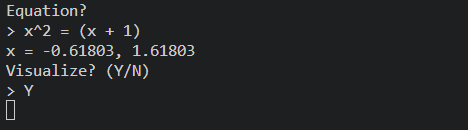
\includegraphics[scale=0.65]{ex1.png}
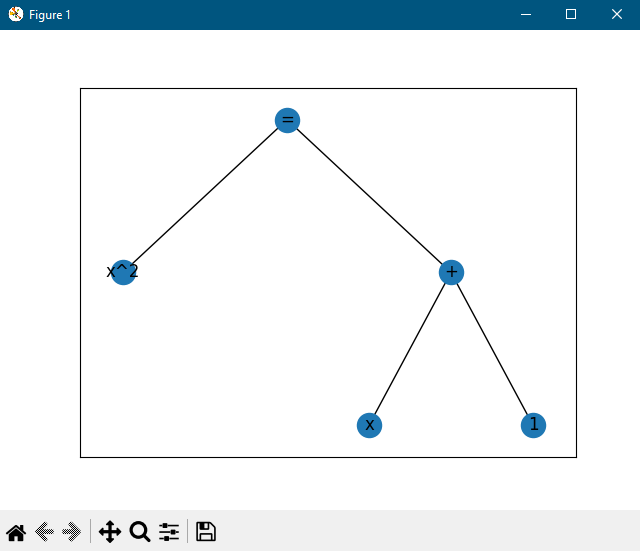
\includegraphics[scale=0.5]{ex2.png}
\end{center}

\section*{Changes From Proposal}

The core of my project has remained the same from what I had initially proposed: a computer algebra system capable of parsing string inputs, solving some classes of equations, and visualizing the equation trees. One notable difference is the realization that creating a computer algebra system capable of solving quadratic equations is complex enough to base our whole project around. As per the feedback we received on the proposal, we also elaborated on the definition of a computer algebra system in this report.

\section*{Discussion}

Our final project achieves the goal mentioned at the top of this report, although the complexity of the program makes it difficult to verify our system on every single valid input. The most complex function in our project is \code{Unit.simplify} (including its helpers), so one major difficulty was determining whether or not it our implementation really satisfies its specifications. It is paramount to our equation-solving algorithm that \code{Unit.simplify} results in a canonical form (see our discussion above), as \code{Equation.solve} relies on the ability to subtract the entire right-hand side from the left-hand side and evaluate solutions based on the resulting coefficients. 

We also found it surprisingly difficult to implement the solution visualization. One major problem was figuring out how to create vertices with duplicate names. Our solution--to assign unique integer identifiers to each vertex, and use a dictionary mapping ids to labels--is imperfect because it makes it difficult to keep track of which vertices belong to which parts of the overall equation. For this reason, the final visualization only displays the part of the equation currently being operated on by the solution algorithm, as opposed to a wholistic view of the manipulations occuring on the initial equation tree. There were also issues with transitioning from one tree to the next, which resulted in the user having to close the GUI at every step, as well as the inability to halt the visualization once it was started.

One other drawback to our computer algebra system is its lack of generality. That is, there is no easy way to implement, say, logarithms or exponential equations into our existing framework, as our solution algorithm relies heavily on the properties of polynomials. This is one way in which we did not reach our original goal from our proposal, since we were hoping to be able to solve more than just polynomial equations. However, as we mentioned under Changes From Proposal, we realized that quadratic equations are themselves quite sophisticated, so we are nonetheless happy to be able to solve this small class of equations.

\section*{References}

\begin{itemize}
\item Wikipedia contributors. (2023, December 20). Computer algebra system. Wikipedia. Retrieved March 3 2024, from \href{https://en.wikipedia.org/wiki/Computer_algebra_system?oldformat=true}{https://en.wikipedia.org/wiki/Computer_algebra_system?oldformat=true}
\item Solving equations. (n.d.). The University of Texas at Austin, Computer Science. Retrieved March 3, 2024, from \href{https://www.cs.utexas.edu/users/novak/algebra.pdf}{https://www.cs.utexas.edu/users/novak/algebra.pdf}
\item GfG. (2022, May 17). Visualize graphs in Python. GeeksforGeeks. Retrieved March 31, 2024, from \href{https://www.geeksforgeeks.org/visualize-graphs-in-python/}{https://www.geeksforgeeks.org/visualize-graphs-in-python/}
\item Joel. (2015, April 13). Can one get hierarchical graphs from networkx with python 3? Stack Overflow. Retrieved March 31, 2024, from \href{https://stackoverflow.com/a/29597209/2966723}{https://stackoverflow.com/a/29597209/2966723}
\end{itemize}

\end{document}
